% Number 80
% Algebra
% Problem setup - fishermen
% MIT Physics for Teachers LON-CAPA

% Watermark
\AddToShipoutPicture*{\BackgroundPic}

\addtocounter {ProbNum} {1}

%\begin{floatingfigure}[r]{.25\textwidth}
%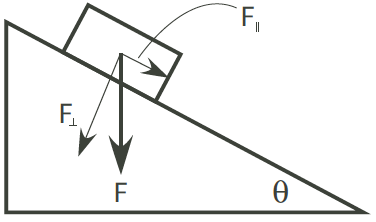
\includegraphics[scale=.4]{/Users/jgates/desktop/latex/pics/inclinedplane2.png}
%\end{floatingfigure}
 
{\bf \Large{\arabic{ProbNum}}} A party of fishermen rented a boat for 240 dollars. Two of the fishermen had to withdraw from the party and, as a result, the share of each of the others was increased by 10 dollars. 

\bigskip

\indent How many were in the original party?  

\vfill

\newpage
